\begin{frame}
    \frametitle{Giróscopo o Giroscopio Mecánico}
    \scriptsize
    \begin{center}
        \movie[autostart,loop,poster]{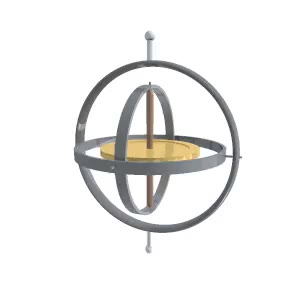
\includegraphics[width=0.25\columnwidth]{./images/gyroscope_video.jpg}}{./videos/gyroscope.mp4}
        \hspace{1em}
        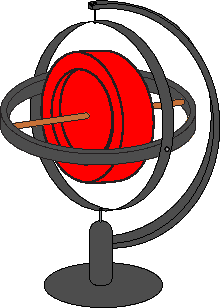
\includegraphics[width=0.15\columnwidth]{images/gyroscope.pdf}
        \hspace{1em}
        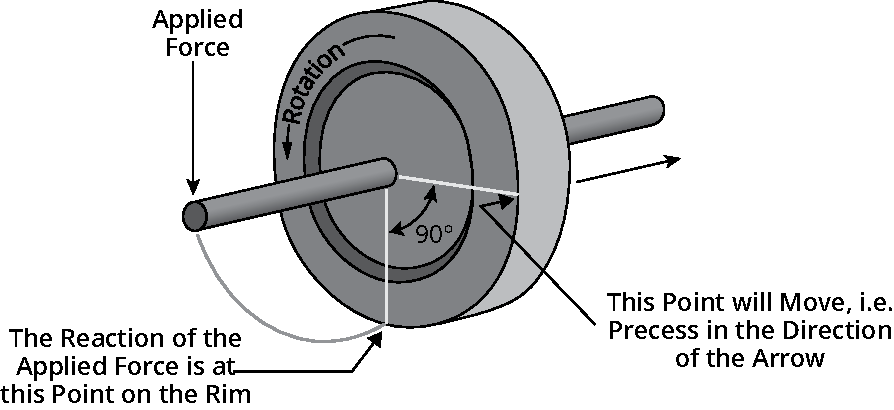
\includegraphics[width=0.4\columnwidth]{images/gyroscope_precession.pdf}
    \end{center}

    \begin{block}{Principio de funcionamiento}
        \begin{itemize}
            \item Un giróscopo mecánico es todo cuerpo simétrico en rotación a una velocidad suficiente como para experimentar los efectos giroscópicos.
            \item Los giróscopos mecánicos son dispositivos que miden o mantienen el movimiento de rotación.
            \item El Giróscopo Mecánico puede ser utilizado para fijar una \textbf{orientación absoluta} haciendo que el disco gire en dicha dirección (utilizando el principio de \textbf{Rigidez en el espacio})
            \item El Giróscopo Mecánico puede ser utilizado para medir \textbf{velocidad angular} (utilizando el principio giroscópico de \textbf{Movimiento de Preseción})
        \end{itemize}
    \end{block}
    
    \TODO{Ver vídeo: https://www.youtube.com/watch?v=V6XSsNAWg00 para extraer sub-videos y aplicaciones (orientación abosuoluta y calculo de velocidad de angular)}

    \note{https://answeringatpl.com/instrumentation/gyroscopic-principles/\\
          https://www.5hertz.com/index.php?route=tutoriales/tutorial&tutorial_id=13
      }

\end{frame}

\begin{frame}
    \frametitle{Giróscopo Mecánico: Principios giroscópicos}
    \note{https://www.youtube.com/watch?v=nhNg-8RSuKY}
    \scriptsize
    
    \begin{center}
        \movie[autostart,loop,poster]{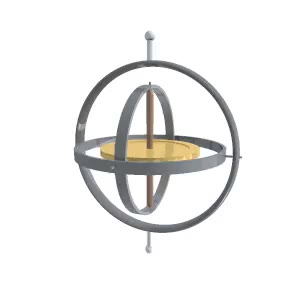
\includegraphics[width=0.25\columnwidth]{./images/gyroscope_video.jpg}}{./videos/gyroscope.mp4}
        \hspace{1em}
        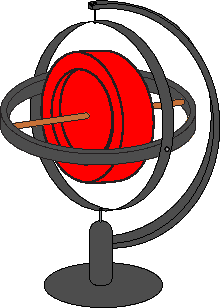
\includegraphics[width=0.15\columnwidth]{images/gyroscope.pdf}
    \end{center}

    \begin{block}{Rigidez en el espacio}
        \begin{itemize}
            \item Al rotar, un giróscopo permanece en una posición fija en su plano de rotación, independientemente del movimiento de los soportes o el marco.
            \item La cantidad de \textbf{rigidez} que presenta el giróscopo es directamente proporcional a su velocidad de rotación (RPM) y su momento de inercia.
            \item Mayor velocidad de rotación, entonces mayor rigidez en el espacio.
            \item Mayor masa y radio efectivo, entonces mayor rigidez en el espacio.
        \end{itemize}
    \end{block}

    \note{Un trompo es un giróscopo! cuando esta por caerse muestra el efecto de precesión. La fuerza que se le aplica es la de la gravedad y hace que se mueva realizando una circunsferencia con su eje.}
\end{frame}


\begin{frame}
    \frametitle{Giróscopo Mecánico: Principios giroscópicos}
    \note{https://www.youtube.com/watch?v=nhNg-8RSuKY}
    \scriptsize
    
    \begin{center}
        \movie[autostart,loop,poster]{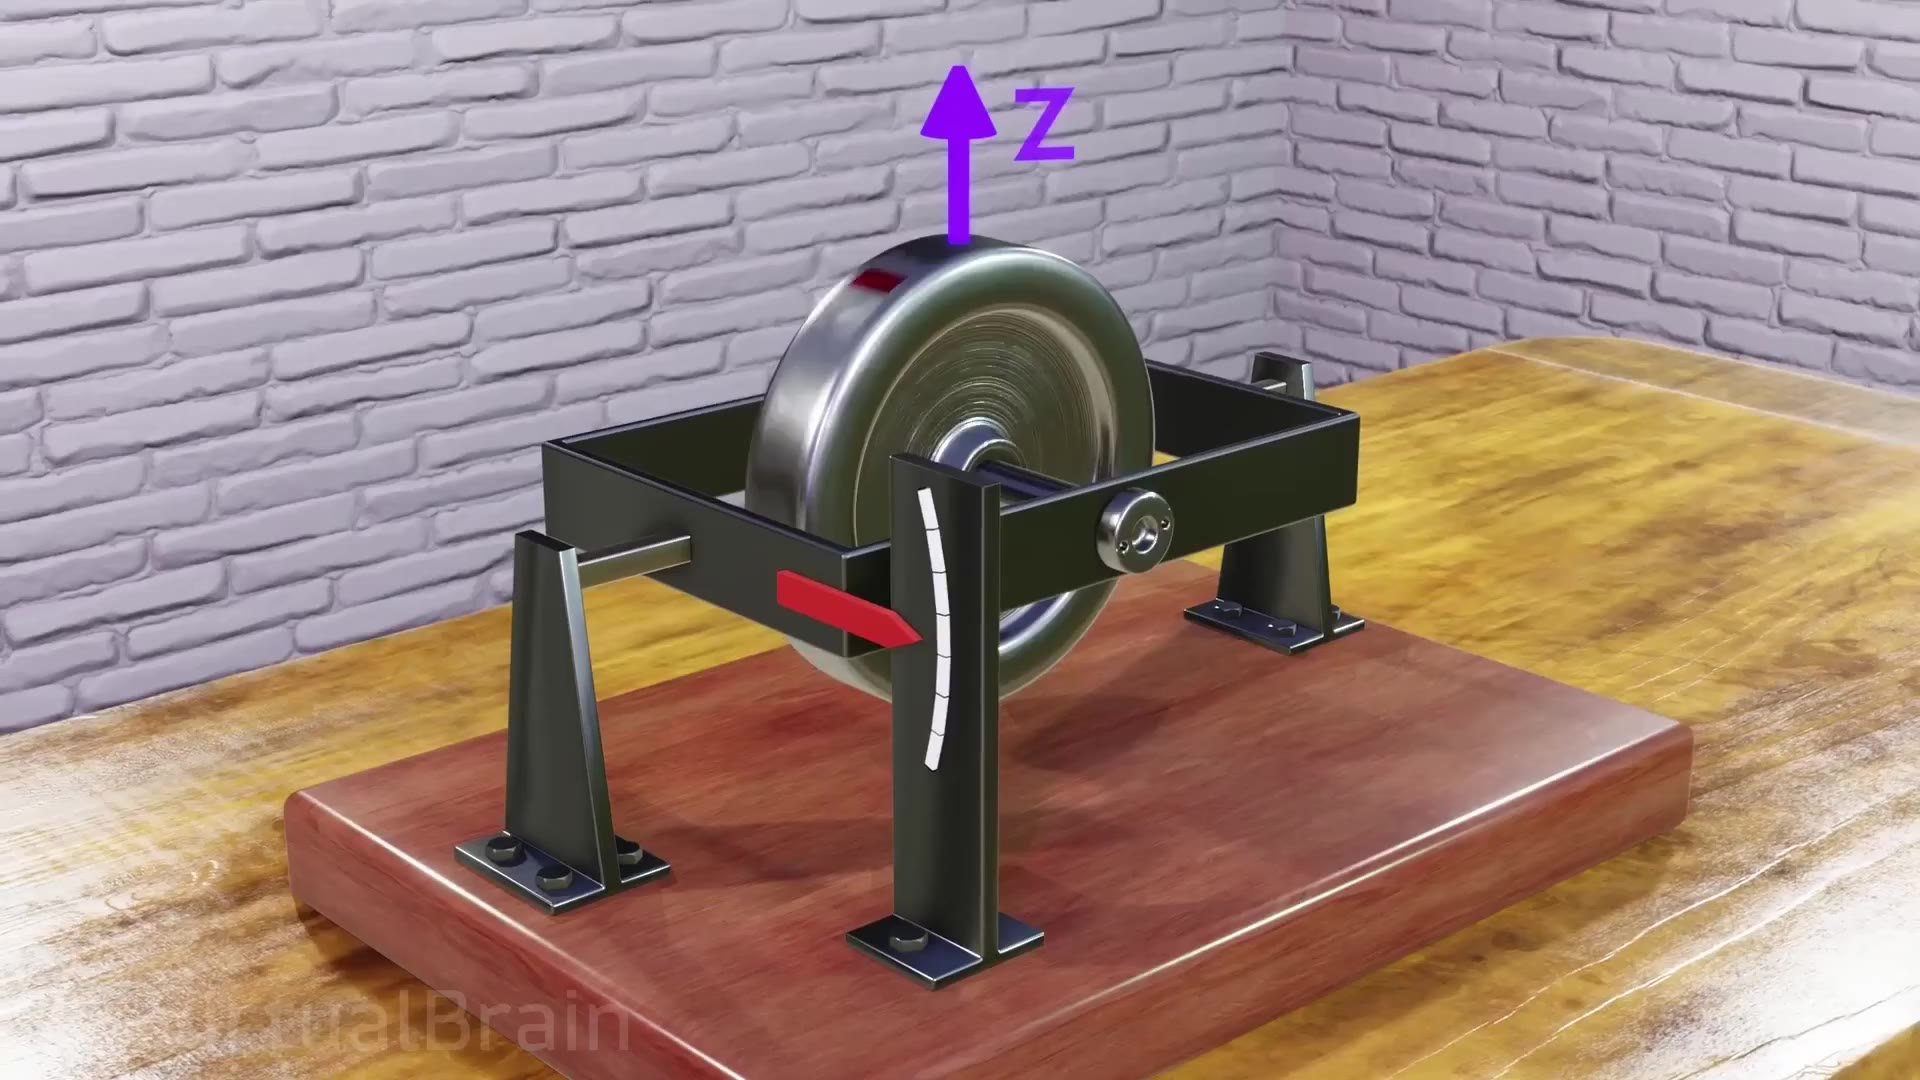
\includegraphics[width=0.5\columnwidth,valign=m]{./images/mechanical_gyroscope_angular_velocity.jpg}}{./videos/mechanical_gyroscope_angular_velocity.mp4}
        \hspace{1em}
        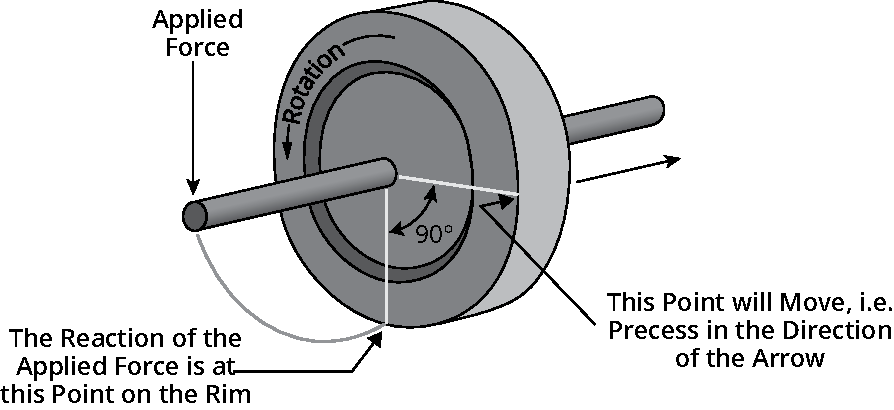
\includegraphics[width=0.4\columnwidth,valign=m]{images/gyroscope_precession.pdf}
    \end{center}
    \begin{block}{Movimiento de Precesión}
            \begin{itemize}
                \item Toda fuerza aplicada perpendicularmente sobre el plano de rotación de un giróscopo se verá reflejada a $\SI{90}{\degree}$ en el sentido de la rotación.
                \item La magnitud de la precesión que presenta el giróscopo es directamente proporcional a la fuerza aplicada e inversamente proporcional a la velocidad de rotación (RPM).
            \end{itemize}
    \end{block}
    
    \note{Un trompo es un giróscopo! cuando esta por caerse muestra el efecto de precesión. La fuerza que se le aplica es la de la gravedad y hace que se mueva realizando una circunsferencia con su eje.}
\end{frame}



\begin{frame}
    \frametitle{Giróscopo MEMS: Aceleración de Coriolis}
    \note{https://www.analog.com/en/technical-articles/mems-gyroscope-provides-precision-inertial-sensing.html}
    \footnotesize
    
    \begin{figure}
        \subfloat[]
        {
            \movie[autostart,loop,poster]{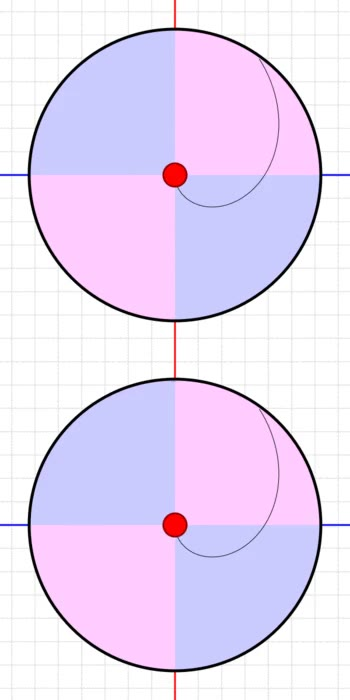
\includegraphics[width=0.1\columnwidth,valign=m]{./images/coriolis_force_video.jpg}}{./videos/coriolis_force.mp4}
        }
        \hspace{2em}
        \subfloat[]
        {
            \movie[autostart,loop,poster]{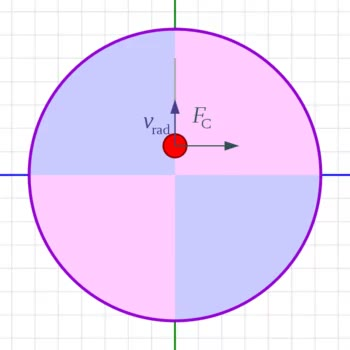
\includegraphics[width=0.2\columnwidth,valign=m]{./images/coriolis_force2_video.jpg}}{./videos/coriolis_force2.mp4}
        }
        \hspace{2em}
        \subfloat[]
        {
            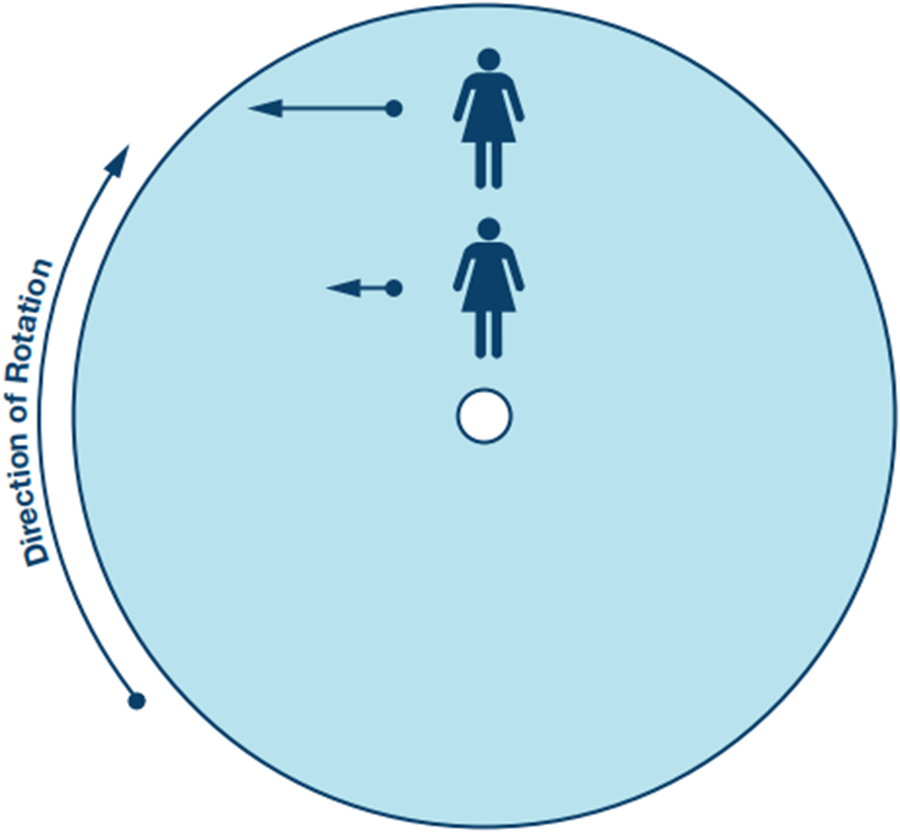
\includegraphics[width=0.2\columnwidth,valign=m]{images/gyroscope_mems_1.png}
        }
    \end{figure}
    
    \begin{block}{Principio de Funcionamiento}
        Los giróscopos MEMS utilizan la \textbf{fuerza de Coriolis}, fuerza tangencial experimentada por un objeto giratorio en movimiento radial.
    \end{block}

    Ejemplo de aceleración de Coriolis:
    Una persona que se mueve hacia el borde exterior Norte de una plataforma giratoria en sentido horario, debe aumentar el componente de velocidad hacia el Oeste (flechas azules) para mantener su rumbo hacia el Norte. La aceleración requerida es la \textbf{aceleración de Coriolis}.
    
    
    \note{Si $\Omega$ es la velocidad angular y $r$ es el radio, la velocidad tangencial es $\Omega r$. Entonces, si $r$ cambia con una velocidad $v$, habrá una aceleración tangencial $\Omega v$. Esta es la mitad de la aceleración de Coriolis. Falta otra mitad para cambiar la dirección de la velocidad radial dando un total de $2 \Omega v$. Si tiene una masa ($M$), la plataforma debe aplicar una fuerza ($2 M \Omega v$) para provocar esa aceleración, y la masa experimenta una fuerza correspondiente de reacción. El Giróscopo aprovecha este efecto utilizando una masa resonante análoga a la persona que se dirige hacia adentro y fuera de una plataforma giratoria. La masa está micromecanizada a partir de polisilicio y está unida a un marco de polisilicio para que pueda resonar sólo en una dirección.}

    \note{Considérese parado en una plataforma giratoria, cerca del centro. Su velocidad relativa al suelo se muestra como la longitud de la flecha azul. Si tuviera que moverse a un punto cerca del borde exterior de la plataforma, su velocidad aumentaría en relación con el suelo, como lo indica la flecha azul más larga. La tasa de aumento de su velocidad tangencial, causada por su velocidad radial, es la aceleración de Coriolis.}

    \note{Los giróscopos MEMS (sistemas microelectromecánicos) son pequeños sensores, de bajo costo para medir la velocidad angular.  El sensor MEMS dentro de un giroscopio es muy pequeño (entre 1 a 100 micrómetros, el tamaño de un cabello humano).}

\end{frame}

\begin{frame}
    \frametitle{Giróscopo MEMS (Microelectromechanical Systems)}

    \note{https://www.analog.com/en/technical-articles/mems-gyroscope-provides-precision-inertial-sensing.html}
    
    \begin{itemize}
        \item Un Giróscopo internamente tiene una masa resonante (vibrando constantemente) dentro de un marco, que permise que solo pueda vibrar en una sola dirección. Este movimiento se convierte en señales eléctricas de muy bajas corrientes que se pueden amplificar para ser leídas por un microcontrolador.
    \end{itemize}
    
    \begin{center}
        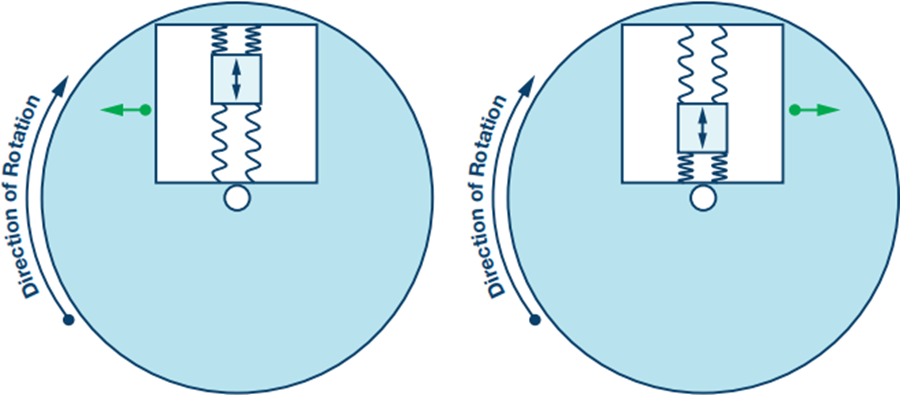
\includegraphics[width=0.4\columnwidth,valign=m]{images/gyroscope_mems_2.png}
        \hspace{1em}
        \movie[autostart,loop,poster]{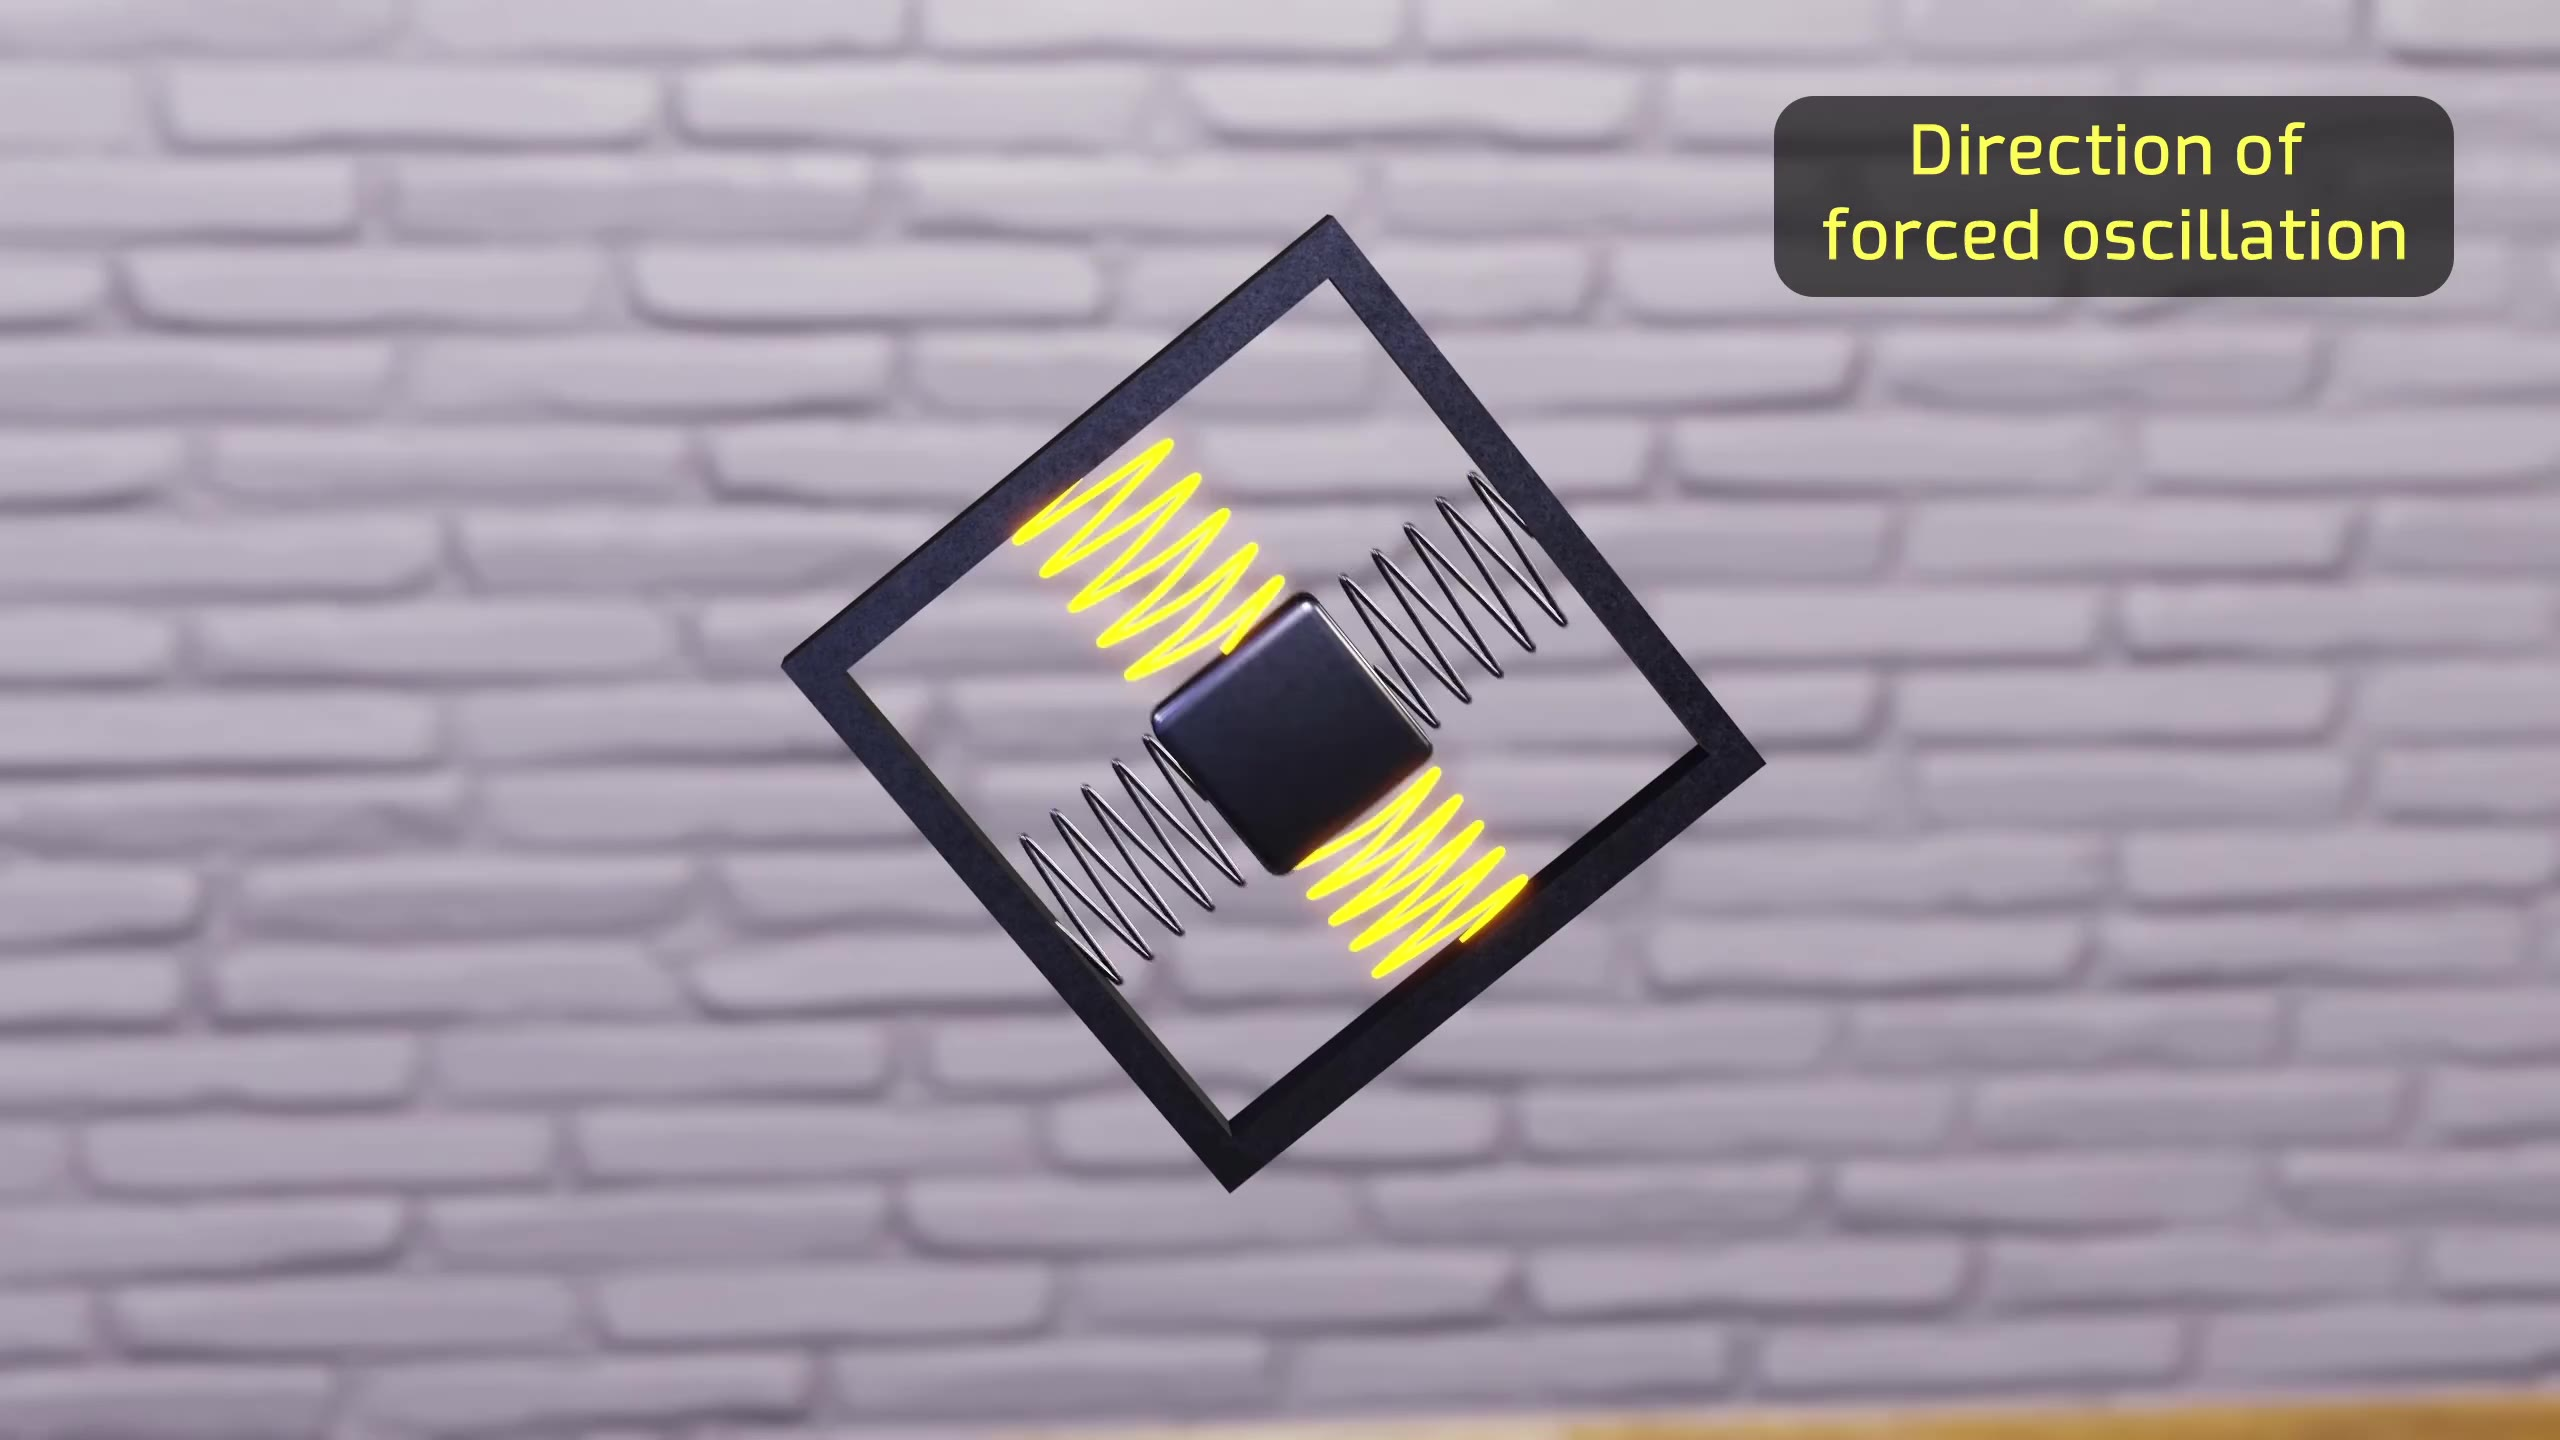
\includegraphics[width=0.4\columnwidth,valign=m]{./images/video_gyroscope_mems.jpg}}{./videos/gyroscope_mems.mp4}
    \end{center}

    \begin{itemize}
        \item Cuando la masa resonante se mueve (o vibra) hacia el borde exterior de la rotación, se acelera hacia la derecha y ejerce sobre el marco una fuerza de reacción hacia la izquierda (flecha verde). Cuando se mueve hacia el centro de la rotación, ejerce una fuerza hacia la derecha (flecha verde).
    \end{itemize}
    
\end{frame}

\begin{frame}
    \frametitle{Giróscopo MEMS (Microelectromechanical Systems)}
    \scriptsize
    \note{https://www.analog.com/en/technical-articles/mems-gyroscope-provides-precision-inertial-sensing.html}

    \begin{figure}[!h]
        \centering
        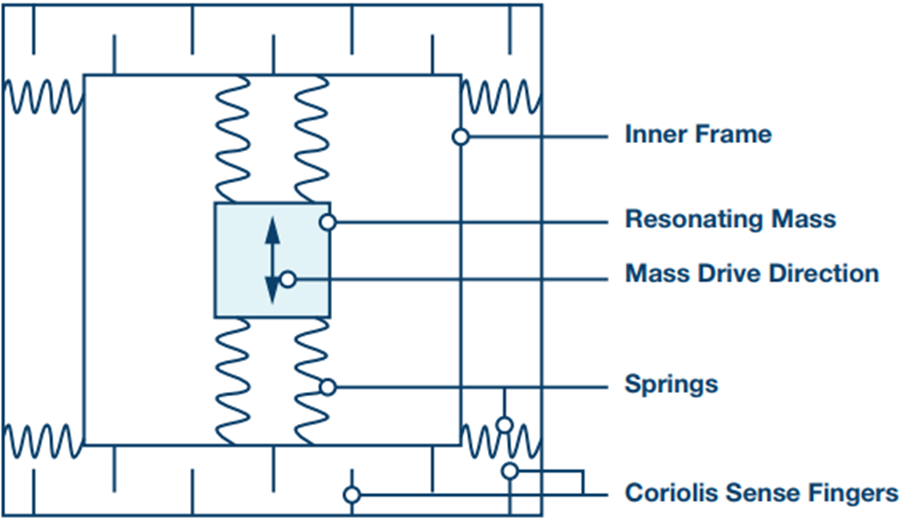
\includegraphics[width=0.5\columnwidth]{images/gyroscope_mems_structure.png}
        \caption{Estructura mecánica de un Giróscopo}
    \end{figure}

    \begin{itemize}
        \item Para medir la aceleración de Coriolis, el marco que contiene la masa resonante está sujeto a un marco externo por resortes a $\SI{90}{\degree}$ en relación con el movimiento resonante (de la masa). Esta figura también muestra los ``dedos'' de detección de Coriolis que se utilizan para detectar el desplazamiento del marco mediante transducción capacitiva en respuesta a la fuerza ejercida por la masa.
    \end{itemize}
\end{frame}

\begin{frame}
    \frametitle{Giróscopo MEMS (Microelectromechanical Systems)}
    \scriptsize
    \note{https://www.analog.com/en/technical-articles/mems-gyroscope-provides-precision-inertial-sensing.html}
        
    \begin{itemize}
        \item A medida que la masa resonante se mueve y la superficie en la que está montado el giróscopo gira, la masa y su marco experimentan la aceleración de Coriolis, y se trasladan $\SI{90}{\degree}$ con respecto al movimiento vibratorio.
        
        \item A medida que aumenta la velocidad de rotación, también aumenta el desplazamiento de la masa y la señal derivada de la capacitancia correspondiente cambia.
    \end{itemize}
    
    \begin{center}
        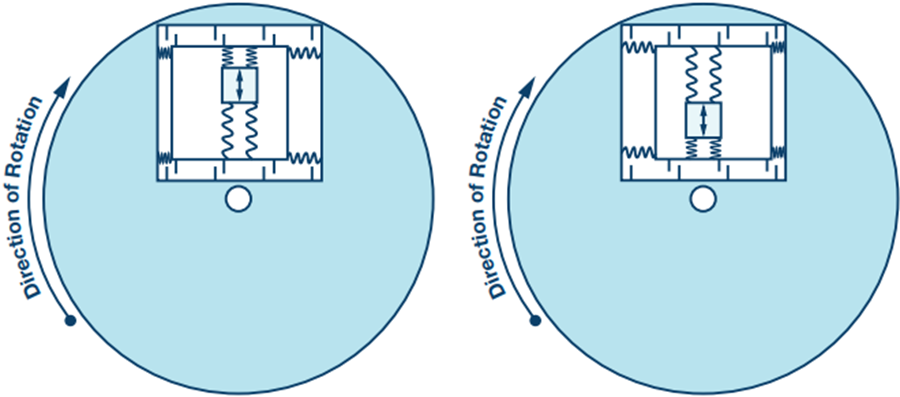
\includegraphics[width=0.5\columnwidth]{images/gyroscope_mems_3.png}
    \end{center}
    
    \begin{center}
        
    \end{center}
    
    \begin{itemize}
        \item Introceptivo
        \item Pasivo
        \item Mide Velocidad Angular
        \item Unidad de medición $\si{\degree\per\second}$ o Revoluciones por Minuto (RPM)
    \end{itemize}

\end{frame}

\begin{frame}
    \frametitle{Giróscopo Óptico: Sagnac Effect}
    \note{Video extraido de https://www.youtube.com/watch?v=V6XSsNAWg00}
    \scriptsize
    
    \TODO{Ver vídeo: https://www.youtube.com/watch?v=V6XSsNAWg00 para extraer sub-videos y aplicaciones (orientación abosuoluta y calculo de velocidad de angular) y giróscopo óptico}
    
\end{frame}


\begin{frame}
    \frametitle{Acelerómetro}
    
    \begin{figure}[!h]
    	\subfloat[]
        {
            \movie[autostart,loop,poster]{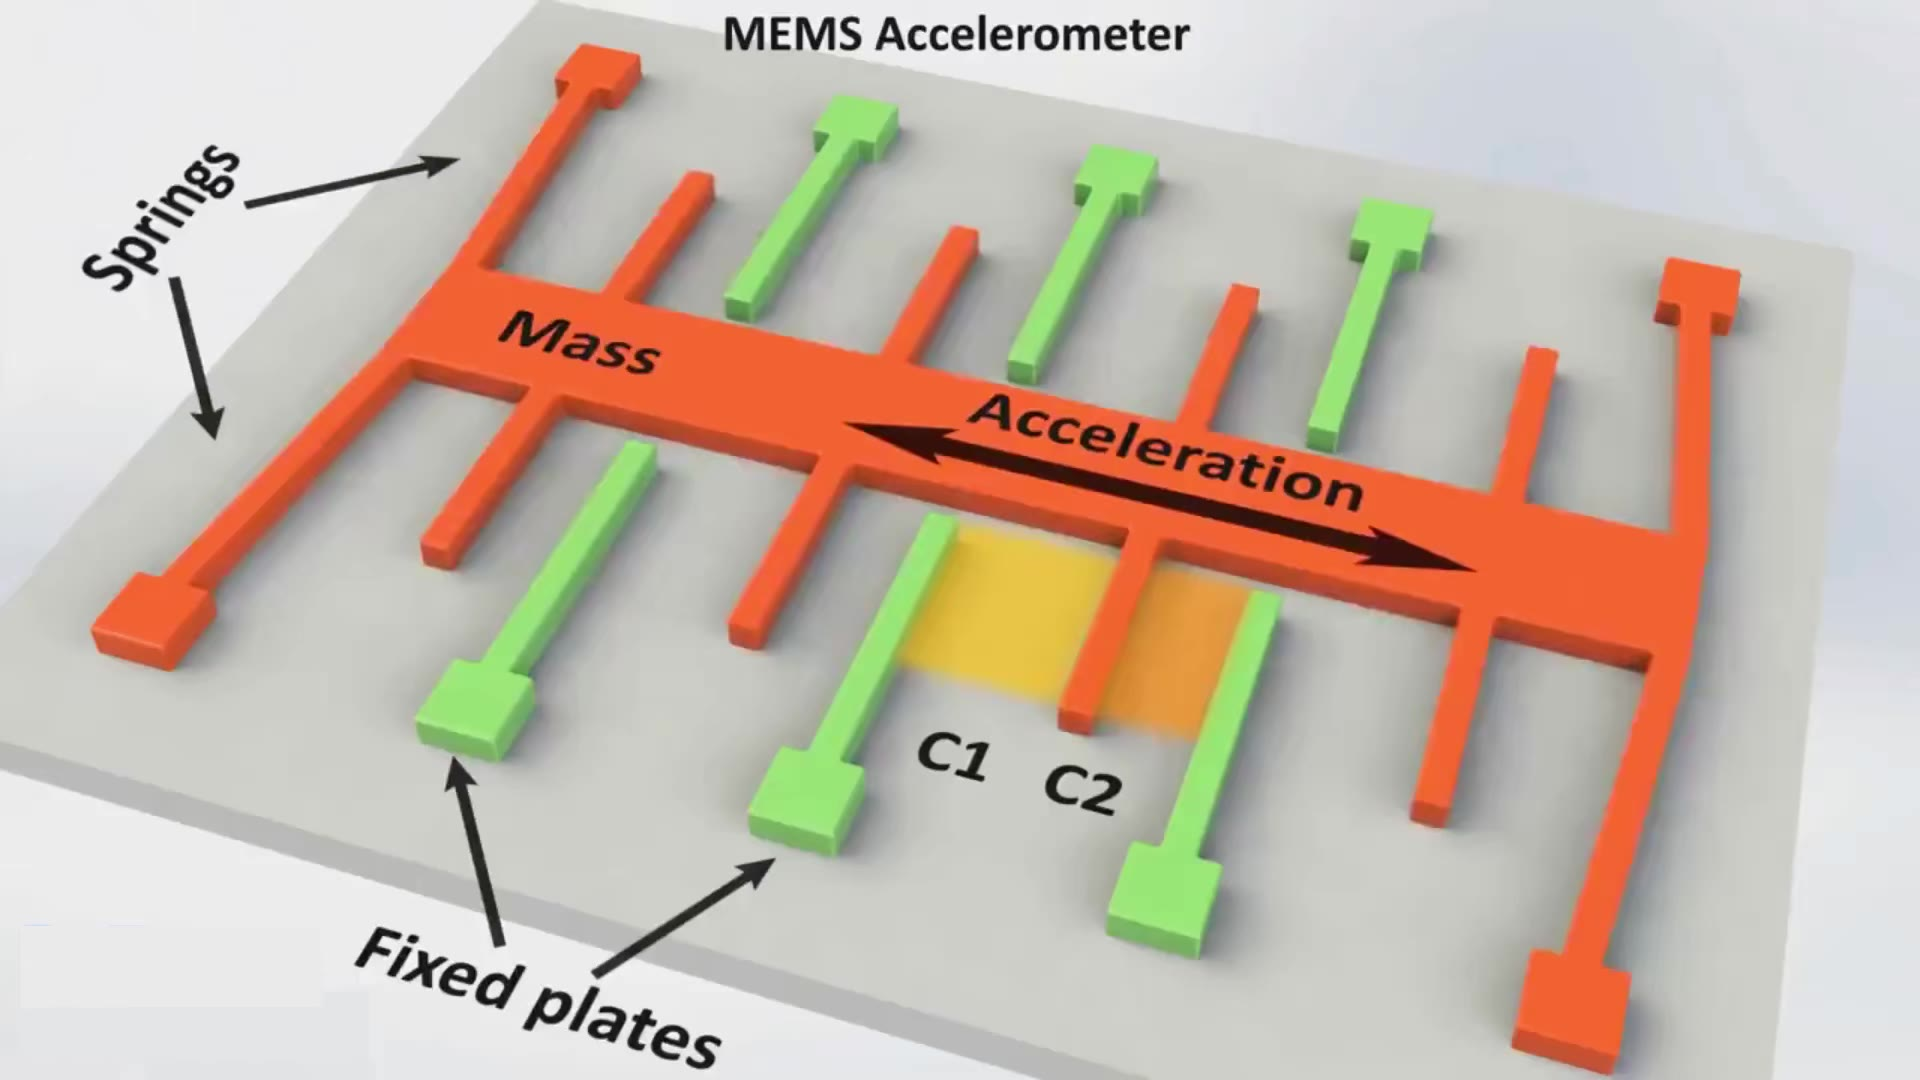
\includegraphics[width=0.3\columnwidth,valign=m]{./images/accelerometer_mems_video.jpg}}{./videos/accelerometer_mems.mp4}
        }
        \hspace{1em}
    	\subfloat[]
    	{
    		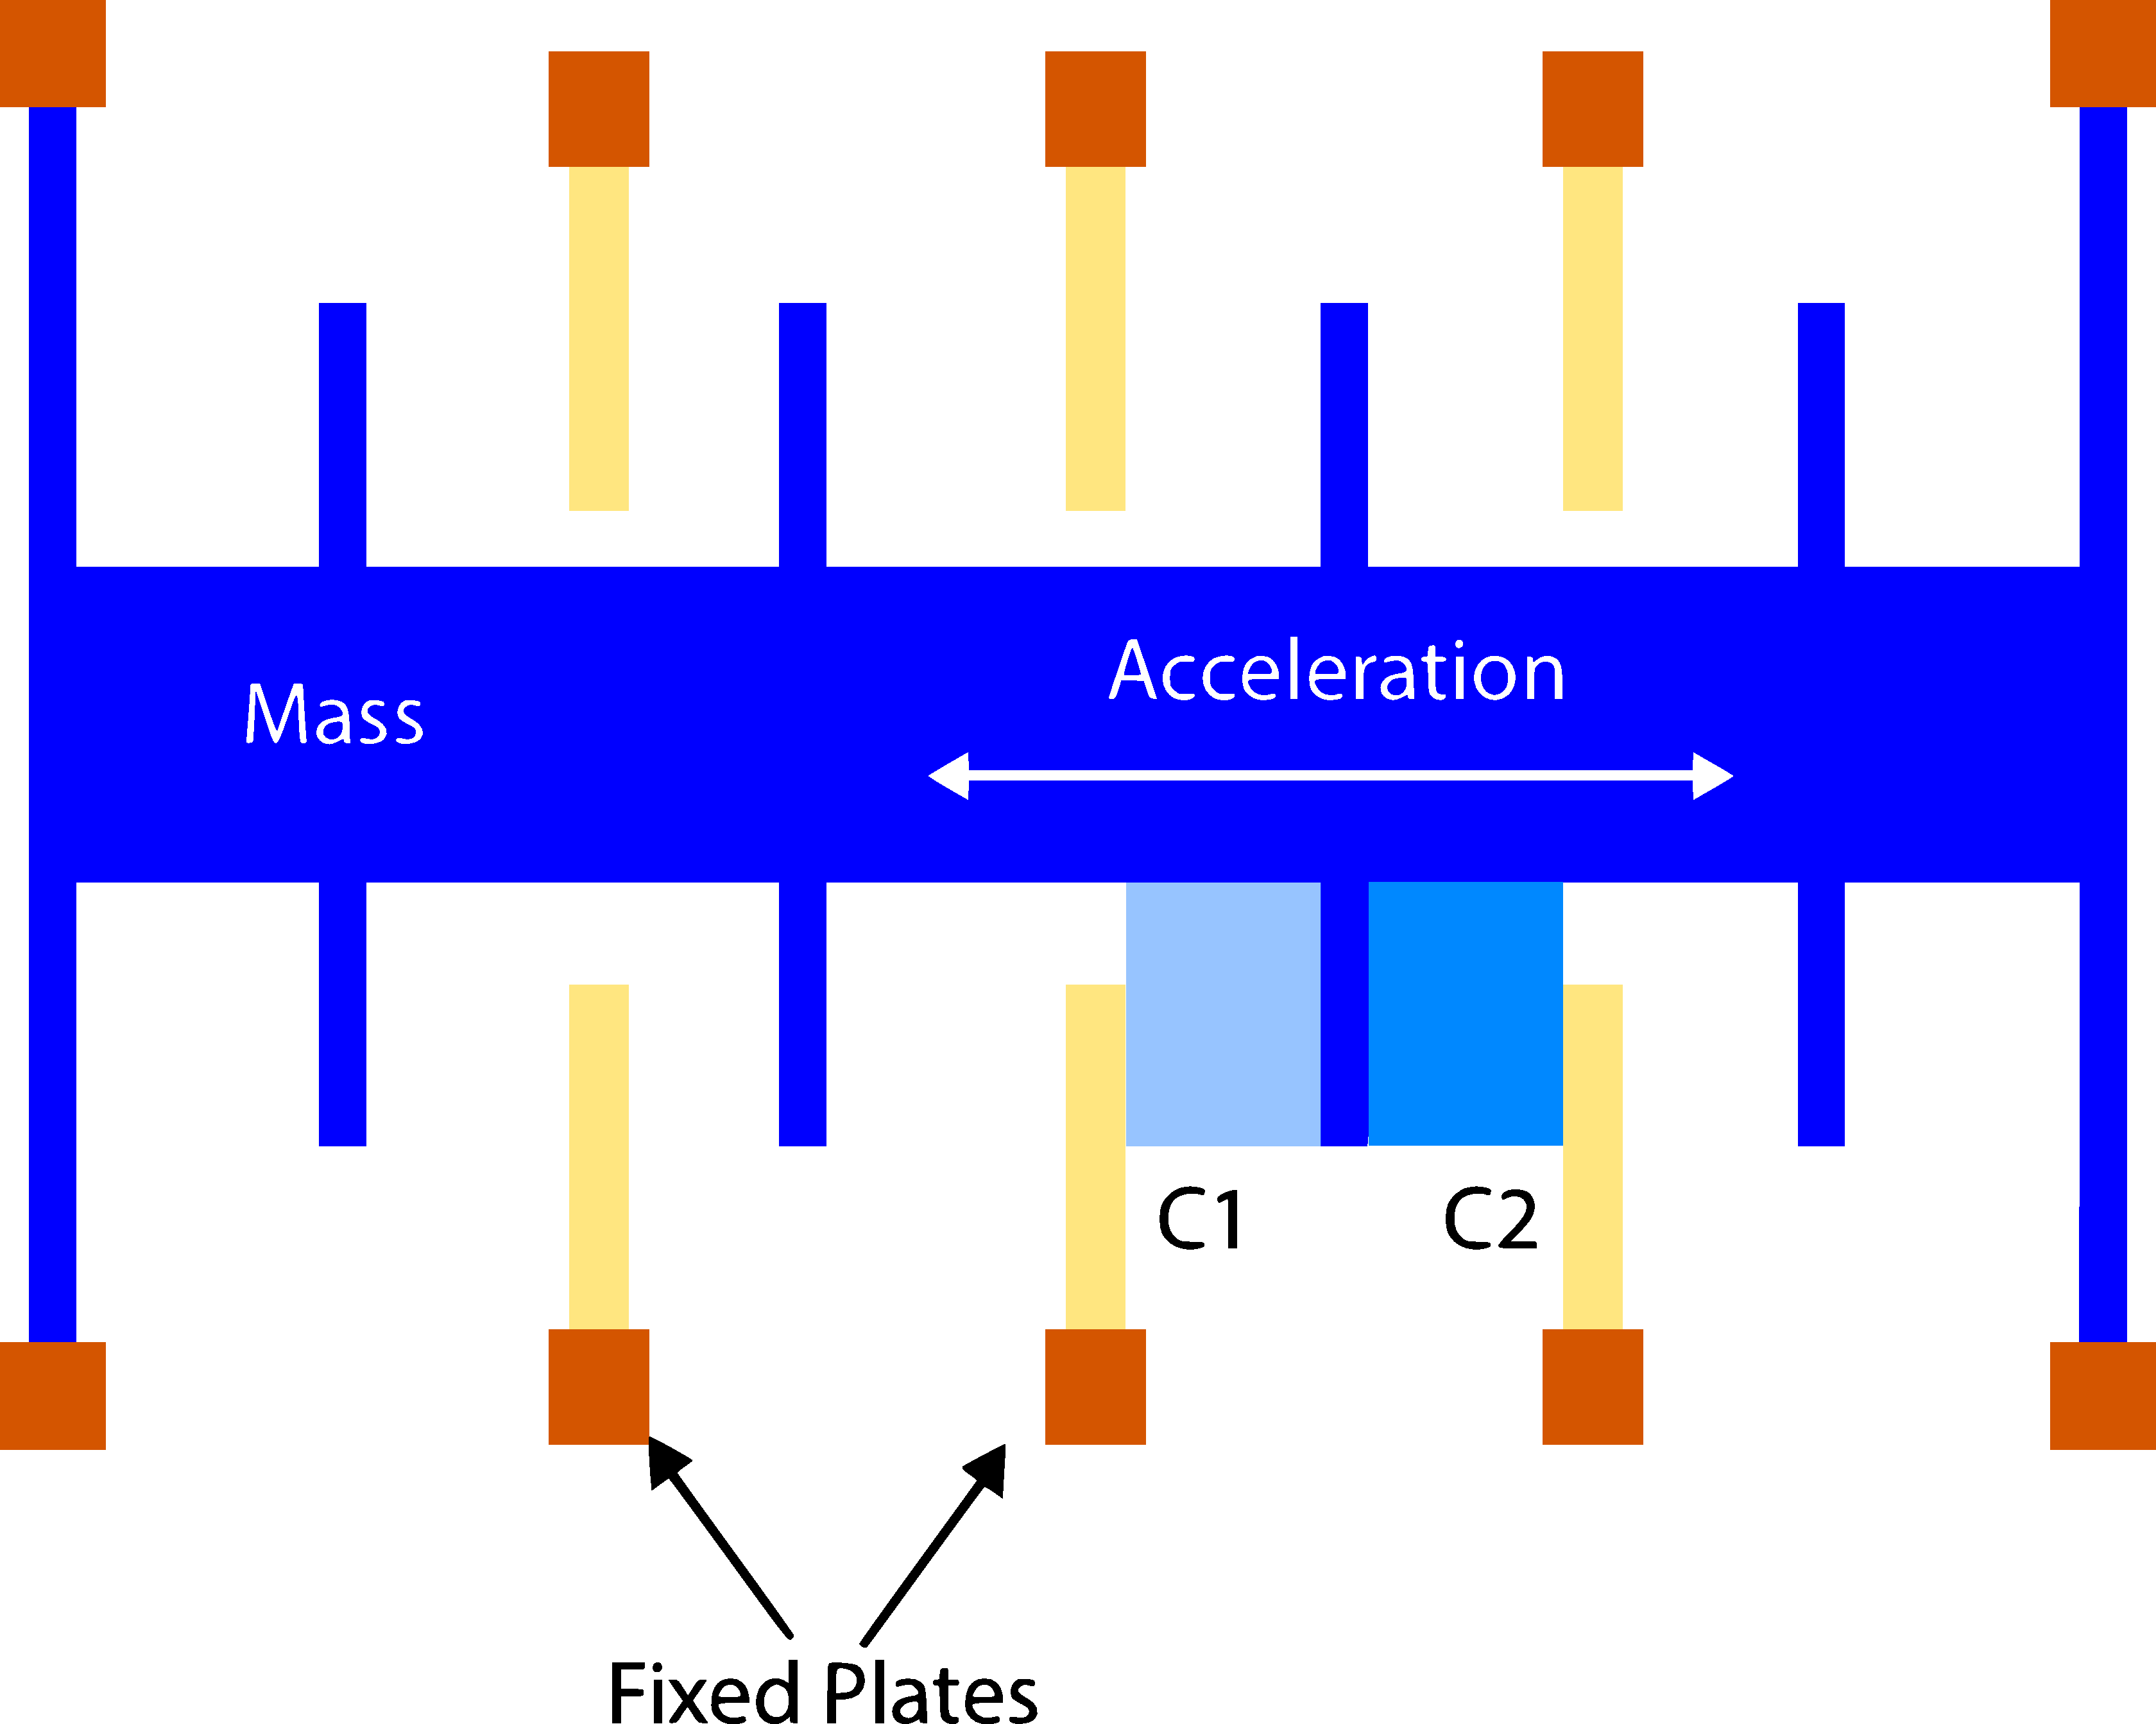
\includegraphics[width=0.2\columnwidth,valign=m]{images/accelerometer_mems.pdf}
    	}
        \hspace{1em}
    	\subfloat[]
    	{
    		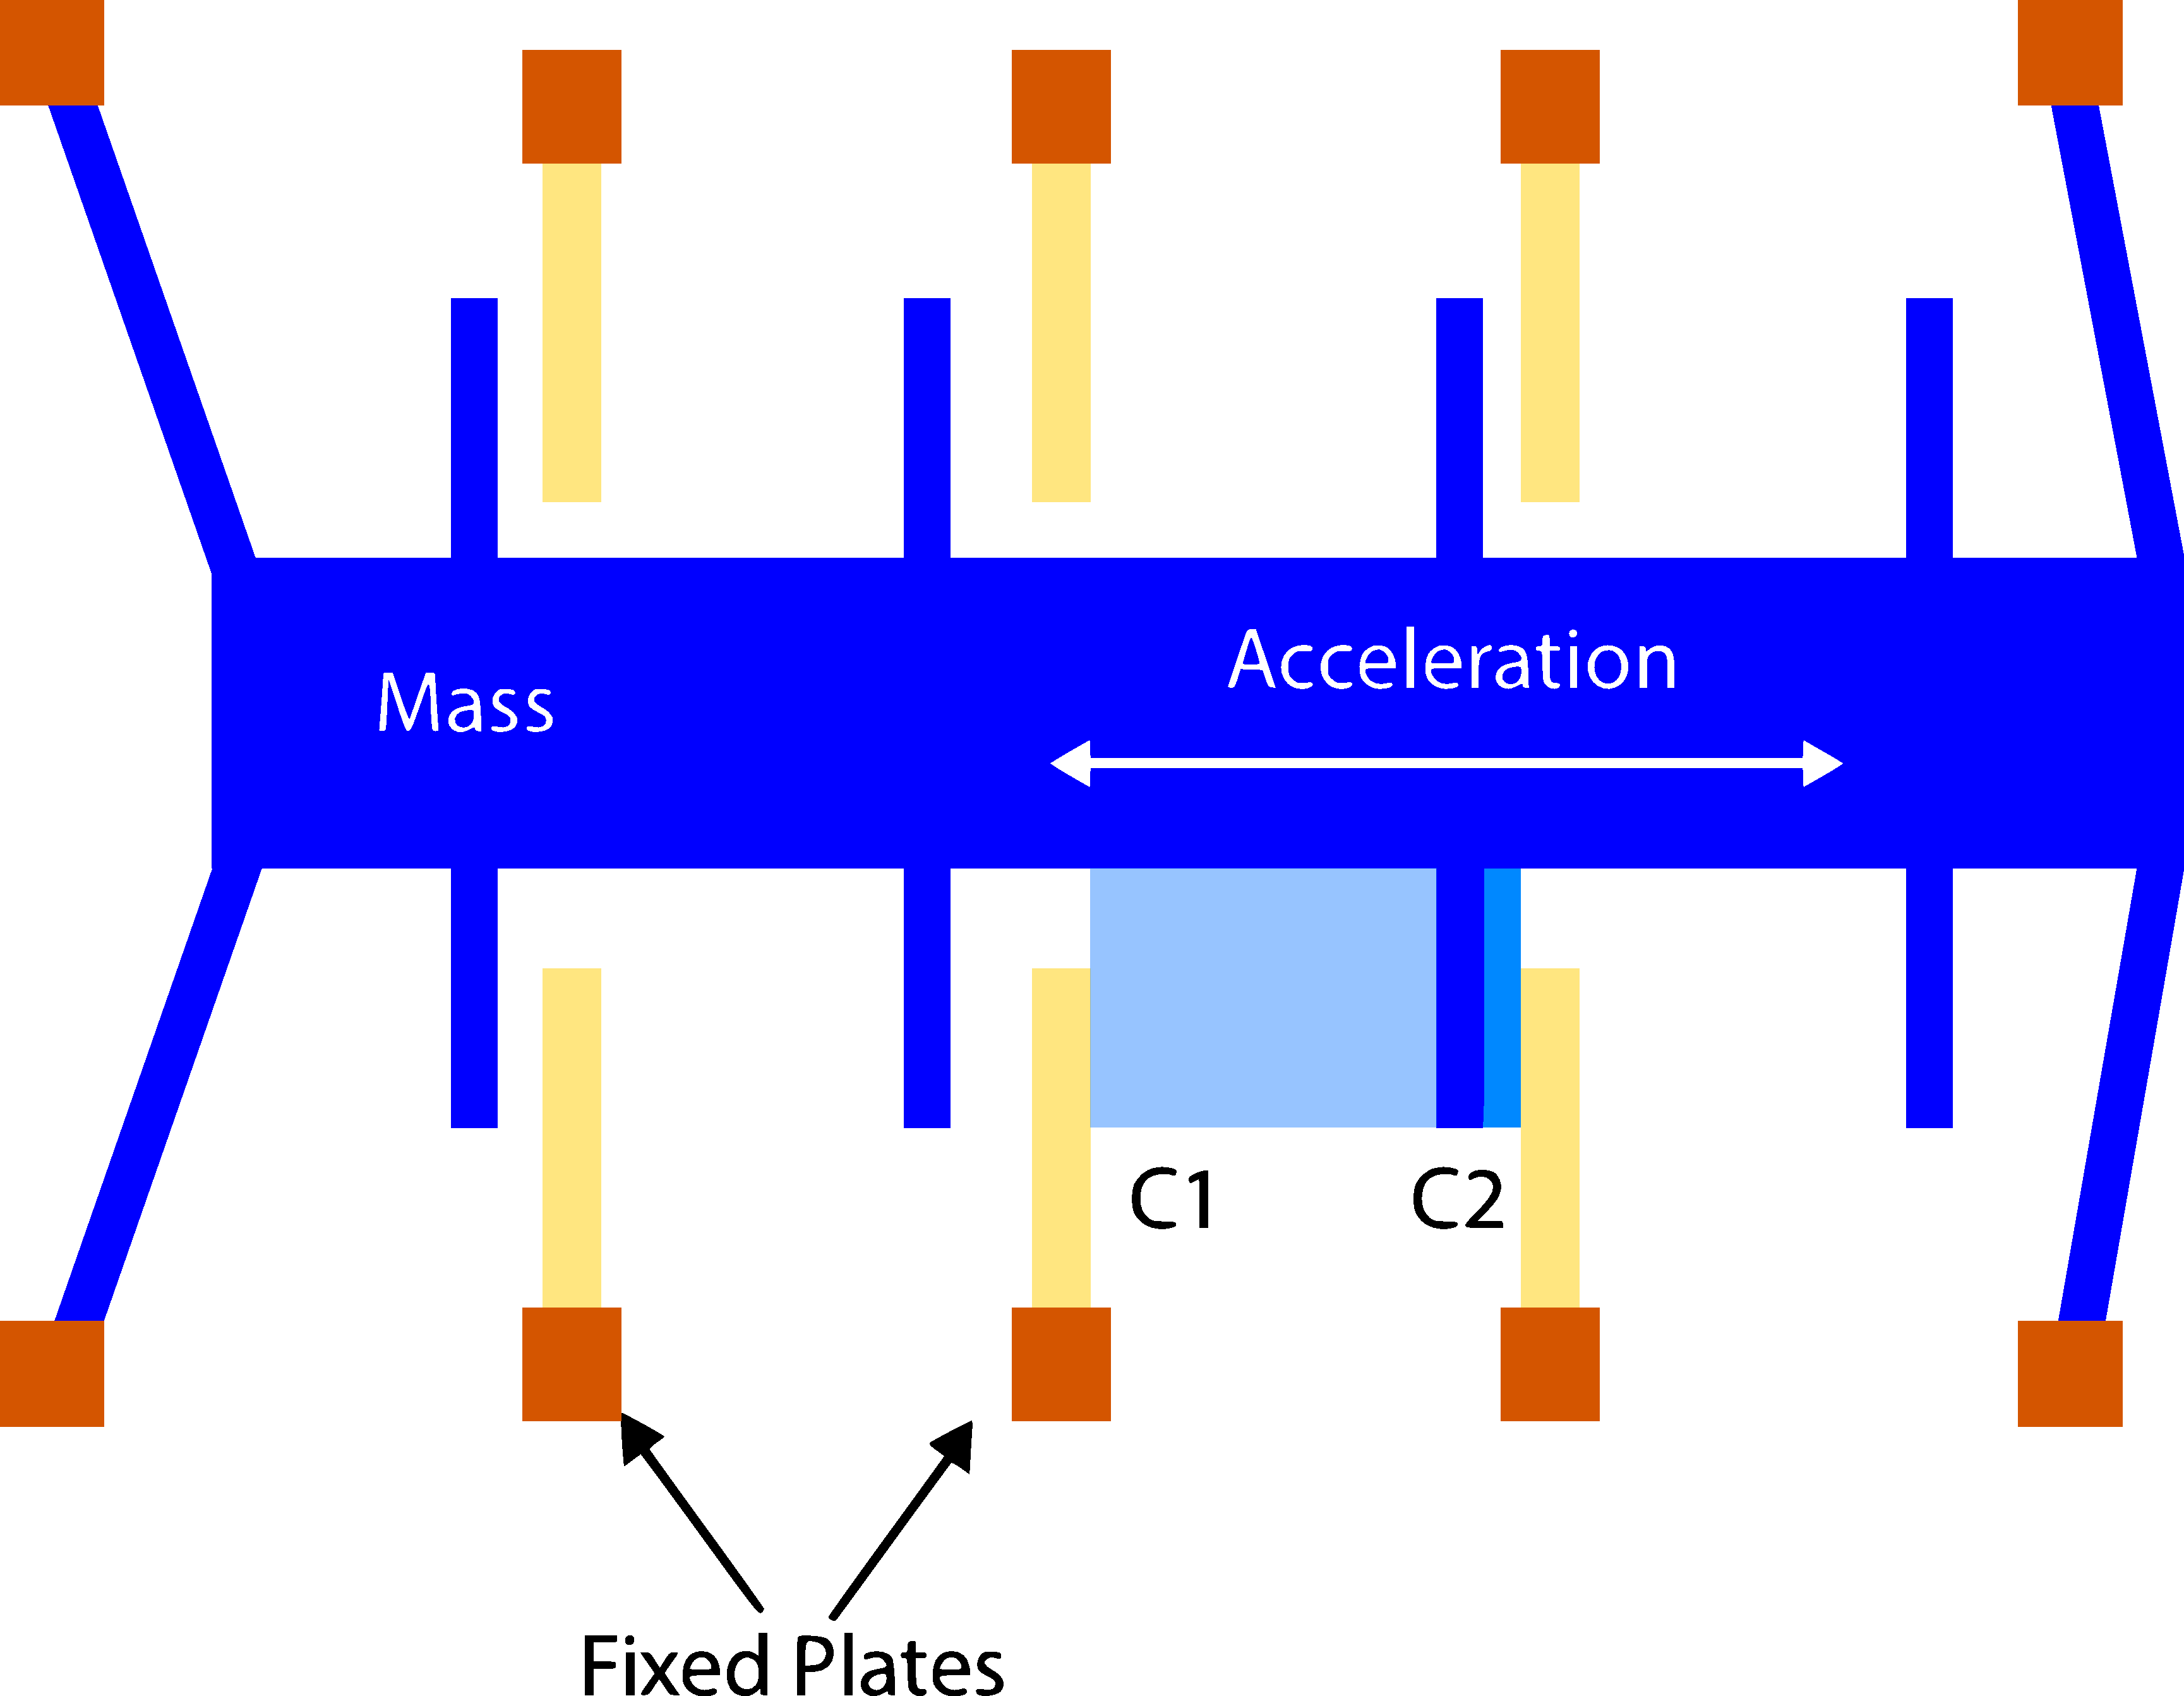
\includegraphics[width=0.2\columnwidth,valign=m]{images/accelerometer_mems2.pdf}
    	}
    \end{figure}
    \scriptsize
    \begin{block}{Principio de Funcionamiento}
        Mide la aceleración midiendo el cambio en la capacitancia. Tiene una masa unida a un resorte que se limita a moverse en una dirección y placas exteriores fijas. Entonces, cuando se aplica una aceleración, la masa se mueve y la capacitancia entre las placas y la masa cambiará. Este cambio de capacitancia es medido, y se corresponde a un valor de aceleración particular.
    \end{block}
    
    \note{La capacitancia es la capacidad de un componente o circuito para recoger y almacenar energía en forma de carga eléctrica.}
    
    \begin{itemize}
        \item Introceptivo
        \item Pasivo
        \item Mide aceleración
        \item Unidad de medición $\si{\meter\per\square\second}$
    \end{itemize}
    
\end{frame}

\begin{frame}
    \frametitle{IMU (Inertial Measurement Unit)}
    \note{página 122 del libro Introduction to autonomous mobile robots 2nd edition}
    
    \begin{figure}[!h]
            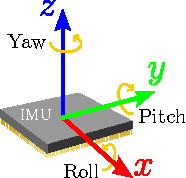
\includegraphics[width=0.2\columnwidth]{images/imu.pdf}
    \end{figure}
    
    \begin{itemize}
        \item 3 giróscopos ortogonales y 3 acelerómetros ortogonales.
        \item Permite estimar: posición, orientación, velocidad lineal, velocidad angular y aceleración 
        \item La orientación se obtiene integrando el giróscopo en el tiempo
        \item La velocidad lineal se obtiene integrando el acelerómetro en el tiempo
        \item La posición se obtiene integrando la velocidad en el tiempo
        \item \textbf{Debido a que los datos del acelerómetro se integran dos veces para obtener la posición, cualquier error residual da como resultado un error cuadrático en la posición}
        \item Mediciones absolutas (GPS o cámaras) permiten cancelar esta deriva de error.
    \end{itemize}
    
    \note{
    Una unidad de medida inercial (IMU) es un dispositivo que utiliza giróscopos y acelerómetros para estimar la posición relativa, la velocidad y la aceleración de un vehículo en movimiento. Una IMU también se conoce como Sistema de Navegación Inercial (INS).
    Una IMU estima la pose de seis grados de libertad (DOF) del vehículo: posición (x, y, z) y orientación (pitch, yaw, roll). También estima velocidad y aceleración.
    
    Los datos del giroscopio se integran para estimar la orientación del vehículo, mientras que los tres acelerómetros se utilizan para estimar la aceleración instantánea del vehículo. A continuación, la aceleración se transforma en el marco de navegación local por medio de la estimación actual de la orientación del vehículo en relación con la gravedad. En este punto, el vector de gravedad se puede restar de la medición. Luego, la aceleración resultante se integra para obtener la velocidad y luego se integra nuevamente para obtener la posición, siempre que tanto la velocidad inicial como la posición sean conocidas a priori. Para superar la necesidad de conocer la velocidad inicial, la integración generalmente comienza en reposo (es decir, velocidad igual a cero).
    
    Observe que las IMU son extremadamente sensibles a los errores de medición tanto en giroscopios como en acelerómetros. Por ejemplo, la deriva en el giroscopio socava inevitablemente la estimación de la orientación del vehículo en relación con la gravedad, lo que da como resultado una cancelación incorrecta del vector de gravedad. Además, observe que, debido a que los datos del acelerómetro se integran dos veces para obtener la posición, cualquier vector de gravedad residual da como resultado un error cuadrático en la posición. Debido a esto y al hecho de que cualquier otro error se integra con el tiempo, la deriva es un problema fundamental en las IMU. Después de un largo período de funcionamiento, todas las IMU se desvían. Para cancelar esta deriva, se requiere alguna referencia a alguna medida externa.
    }
\end{frame}

